\documentclass[12pt,a4paper]{report}

%------------------------------------------------
% Packages
%------------------------------------------------
\usepackage[a4paper,margin=1in]{geometry}
\usepackage{times}
\usepackage{setspace}
\usepackage{titlesec}
\usepackage{tocloft}
\usepackage{graphicx}
\usepackage{caption}
\usepackage{longtable}
\usepackage{array}
\usepackage{booktabs}
\usepackage{enumitem}
\usepackage[hidelinks]{hyperref}

%------------------------------------------------
% Font and spacing
%------------------------------------------------
\renewcommand{\familydefault}{ptm}
\setstretch{1.2}

%------------------------------------------------
% Chapter Formatting (Level 1)
%------------------------------------------------
\titleformat{\chapter}
{\normalfont\fontsize{18}{22}\bfseries\rmfamily\raggedleft}
{CHAPTER \thechapter}
{1em}
{\MakeUppercase}

%------------------------------------------------
% Section Formatting (Level 2)
%------------------------------------------------
\titleformat{\section}
{\normalfont\fontsize{16}{20}\bfseries\rmfamily}
{\thesection}
{1em}
{\MakeUppercase}

%------------------------------------------------
% Subsection Formatting (Level 3)
%------------------------------------------------
\titleformat{\subsection}
{\normalfont\fontsize{14}{18}\bfseries\rmfamily}
{\thesubsection}
{1em}
{}

%------------------------------------------------
% TOC Settings
%------------------------------------------------
\setcounter{tocdepth}{1}

%------------------------------------------------
% Paragraph Formatting
%------------------------------------------------
\setlength{\parskip}{10pt}
\setlength{\parindent}{0pt}

%------------------------------------------------
% Caption Formatting
%------------------------------------------------
\captionsetup{
font=small,
labelfont=bf,
labelsep=colon
}

%------------------------------------------------
% Document
%------------------------------------------------
\begin{document}

%------------------------------------------------
% Title Page
%------------------------------------------------
\begin{titlepage}
\centering
\vspace*{1.5cm}

{\Huge\bfseries Namal University Mianwali\\[0.5cm]}
{\Large Department of Computer Science\\[1cm]}
\begin{figure}
    \centering
    \includegraphics[width=0.5\linewidth]{logo.jpg}
\end{figure}



{\LARGE\bfseries Vehicle Transport Management System\\[0.3cm]}


\textbf{Prepared by:}\\[0.5cm]

\begin{tabular}{@{} l @{\hspace{3cm}} r @{}}
\textbf{Name} & \textbf{Roll No} \\[0.3cm]
Tahira Hanif & NUM-BSCS2024-16 \\
Momina Umar & NUM-BSCS2024-36 \\
Mubashir Aman & NUM-BSCS2024-37 \\
\end{tabular}

\vspace{1.5cm}

\begin{spacing}{1.1}
\textbf{Course:} Database\\
\textbf{Instructor:} Asia Batool
\end{spacing}

\vspace{1.5cm}

\textbf{Date:} \today

\vfill
\end{titlepage}

%------------------------------------------------
% Table of Contents
%------------------------------------------------
\tableofcontents
\newpage

%------------------------------------------------
% Revision History
%------------------------------------------------
\chapter*{REVISION HISTORY}

\begin{longtable}{|p{3cm}|p{2cm}|p{6cm}|p{3cm}|}
\hline
\textbf{Date} & \textbf{Version} & \textbf{Description} & \textbf{Approved By} \\
\hline
15/04/2026 & V 1.0 & Initial submission of the VTMS Database Design Document for academic evaluation. & Asia Batool \\
\hline
\end{longtable}

%------------------------------------------------
% CHAPTER 1
%------------------------------------------------
\chapter{PROJECT OVERVIEW}

\section{INTRODUCTION}

 Efficient vehicle transportation is essential for businesses that handle vehicle export services. Delivering on time, keeping accurate records, and coordinating well between departments are important factors for smooth operations and customer's satisfaction. However, many companies still use manual methods like record books or simple spreadsheets to manage their transportation tasks. These old-fashioned ways can lead to lost data, repeated records, delays in processing orders, and problems with tracking shipments.
To solve these issues, we propose a Vehicle Transport Management System (VTMS) that brings in a computerized, database driven approach to managing vehicle transportation. This system will keep and manage all operational data in a structured database, making it easy to store, retrieve, and handle transportation related information.
The VTMS will offer several important features like selecting vehicle types, placing orders, tracking shipments and processing payments. It will also use Role-Based Access Control (RBAC) to ensure that users can access the system based on their roles. The main users will include vehicle buyers, administrators, transport managers, and finance managers.
By using a centralized database with MySQL, the system will improve data accuracy, cut down on duplicate records, and provide secure management of transportation information. Additionally, it will give real-time updates on shipment status through unique tracking IDs and automatic notifications. Overall, the Vehicle Transport Management System will offer a reliable, efficient, and scalable way to manage vehicle transportation operations in today's digital world.

\section{PROBLEM STATEMENT}

Vehicle buyers in Pakistan often face difficulties arranging reliable and timely transportation for their purchased vehicles. Existing transport services do not have a centralized system to manage shipments efficiently. This lack of coordination causes delays, inaccurate fee calculations, and limited transparency. Customers cannot easily track their vehicles in real time or verify deliveries securely. Payments and refunds are often unclear or handled inconsistently.
Transportation companies also face challenges. They struggle to manage available trucks and drivers. Coordinating shipment assignments and maintaining accurate records of vehicles, payments, and customer information is difficult. These issues lead to missed shipments, underused resources, and low customer satisfaction.
The Vehicle Transport Management System (VTMS) will solve these problems. The system allows customers to book shipments, calculate fees automatically, and make payments securely. It verifies deliveries using OTP and tracks shipments in real time. The system also manages trucks and drivers efficiently. It stores accurate data and provides clear records. VTMS improves transparency, reliability, and the overall efficiency of domestic vehicle transportation services.

\section{PROJECT OBJECTIVES}

The primary objective of this project is to design and implement a database-driven Vehicle Transport Management System (VTMS) that efficiently manages vehicle transportation operations by storing, organizing, and processing all data related to vehicle orders, customers, shipments, and payments. The system replaces traditional manual record-keeping with a centralized MySQL database that ensures accurate tracking of all transportation activities, improves data management, and enhances coordination among all stakeholders in the vehicle transport process.

The specific objectives of the VTMS are as follows:
\begin{itemize}
    \item \textbf{Enable Online Shipment Booking: }Allow customers to book vehicle shipments without prior registration. A unique CustomerID is auto-generated from the customer's phone number or email at the time of booking. Booking details including VehicleID, ShipmentType, pickup and delivery locations, and booking date are stored securely in the Shipment table of the database
      \item \textbf{Calculate Shipment Fees Automatically:} Determine accurate fees based on vehicle category, shipment type, and distance using Google Maps API. Store the calculated fee in the database and display it transparently to the customer.
      
      \item \textbf{Handle Payments Efficiently:} Support advance and cash-on-delivery payments. Record all payment transactions in the database, track their status, and enforce the refund policy at the booking stage.
    
    \item \textbf{Verify Customers and Deliveries via OTP:} Generate unique OTPs at the time of booking and at the time of delivery confirmation. Store OTP records in the OTP table with fields for OTPID, ShipmentID, CustomerID, OTP\_Value, Generated\_Time, Expiry\_Time, Verification\_Status, Purpose, and VerifiedAt. Prevent confirmation if the OTP is expired or invalid.
    
     \item \textbf{Track Shipments:} Maintain a complete Shipment\_Status\_Log for every shipment, recording Old\_Status, New\_Status, ChangedBy, Changed\_Time, Notes, and Current\_Location at each status transition (Booked → Scheduled → In Transit → Delivered). Provide both customers and transport managers with access to current shipment status and ETA.
    \item \textbf{Manage Trucks, Drivers, and Driver Assignments: }Maintain up-to-date Truck and Driver records in the database. Use the Driver\_Assignment table (with fields AssignmentID, DriverID, TruckID, Assignment\_Date, End\_Date, and Status) to manage which driver and truck are assigned to each shipment. Allow transport managers to update statuses and handle unavailability by marking shipments as Pending
    \item \textbf{Ensure Data Accuracy and Security:} Store and manage all customer, shipment, vehicle, payment, OTP, and notification data reliably in MySQL. Implement Role-Based Access Control (RBAC) via the User table, restricting system access to authorized roles: Transport Manager, Finance Manager, Driver, and Admin.
     \item \textbf{Support Operational Transparency:} Generate unique TrackingIDs for every shipment. Record all shipment status changes in the Shipment\_Status\_Log and all notifications in the Notification table. Produce operational and financial reports that support monitoring, auditing, and decision-making across the organization.
\end{itemize}

GitHub Repository: \url{https://github.com/MominaUmar74/VTMS.git}

%------------------------------------------------
% CHAPTER 2
%------------------------------------------------
\chapter{DETAILED DATABASE DESIGN}

\section{ENTITY}

The following table identifies and defines all entities in the VTMS database. Each entity represents a distinct real world concept central to the vehicle transportation workflow. Associative entities arising from many-to-many relationships (such as Driver\_Assignment) are included here as they appear as named tables in the ERD.

\begin{longtable}{|c|p{4cm}|p{9cm}|}
\hline
\textbf{Sr. No} & \textbf{Entity Name} & \textbf{Description}\\
\hline

01 & Customer & An individual who books a vehicle shipment. CustomerID is auto-generated from phone or email; no pre-registration is required. \\
\hline

02 & User & An internal staff member with a defined system role (Transport Manager, Finance Manager, Driver, or Admin) who accesses the VTMS backend. \\
\hline

03 & Driver & An employee responsible for operating an assigned truck and delivering vehicles. Extends User with license and status details. \\
\hline

04 & Vehicle & The vehicle to be transported. Linked to a Vehicle\_Category and contains make, model, year, color, and registration details. \\
\hline

05 & Vehicle\_Category & A lookup table defining the five vehicle categories (Motorcycle, Sedan, SUV/MPV, Pickup, Luxury) along with their base rate per km and fee multiplier. \\
\hline

06 & Shipment & A vehicle transport order that captures pickup/delivery locations, booking date, distance, fee, shipment status, delivery date, payment status, TrackingID, and AssignmentID. \\
\hline

07 & Truck & A company-owned transport vehicle used to carry customer vehicles. Tracks truck type, capacity, and current operational status. \\
\hline

08 & Driver\_Assignment & An associative entity recording which driver and truck are assigned to a shipment, including assignment date, end date, and assignment status. \\
\hline

09 & Shipment\_Status\_Log & An audit trail table that records every status change for a shipment, including old status, new status, who changed it, timestamp, notes, and current location. \\
\hline

10 & Payment & Records all financial transactions linked to a shipment, including advance and COD payments, refund status, and which staff member processed the transaction. \\
\hline

11 & OTP & Stores one-time passwords generated for booking confirmation and delivery verification, including expiry time and verification result. \\
\hline

12 & Notification & Records all automated messages sent to customers or staff regarding booking, payment, OTP verification, or shipment status updates. \\
\hline

\caption{VTMS Entity Definitions}

\end{longtable}

%------------------------------------------------
% DATA DICTIONARY
%------------------------------------------------
\section{DATA DICTIONARY}

The data dictionary below defines every attribute of each entity identified in the ERD, including data type, constraint, and description. Foreign Keys (FK) are noted in the attribute name and description.

%======================== CUSTOMER ========================

\subsection{Customer}

Stores information about the vehicle owner who places a shipment booking. No pre-registration is required; the CustomerID is generated automatically from the customer's contact details.

\begin{longtable}{|c|p{3.5cm}|p{2.5cm}|p{3.5cm}|p{5cm}|}
\hline
\textbf{Sr. No} & \textbf{Name} & \textbf{Data Type} & \textbf{Constraint} & \textbf{Description} \\
\hline
01 & Customer\_ID (PK) & VARCHAR(20) & NOT NULL, UNIQUE & Auto-generated unique identifier derived from the customer's phone number or email at booking time. \\
\hline
02 & Name & VARCHAR(100) & NOT NULL & Full name of the customer. \\
\hline
03 & Phone & VARCHAR(15) & NOT NULL, UNIQUE & Customer's primary contact phone number; used for OTP delivery. \\
\hline
04 & Email & VARCHAR(100) & UNIQUE, NULL & Customer's email address (optional). \\
\hline
05 & Address & VARCHAR(255) & NULL & Customer's residential or business address for reference. \\
\hline
\end{longtable}

%======================== USER ========================

\subsection{User}

Represents all internal staff members of the transport company. The Role attribute enforces access control through RBAC. The Driver entity is a specialisation of User and shares the same UserID as its primary key

\begin{longtable}{|c|p{3.5cm}|p{2.5cm}|p{3.5cm}|p{5cm}|}
\hline
\textbf{Sr. No} & \textbf{Name} & \textbf{Data Type} & \textbf{Constraint} & \textbf{Description} \\
\hline
01 & UserID (PK) & VARCHAR(15) & NOT NULL, UNIQUE & Unique identifier for each internal system user (staff member). \\
\hline
02 & UserName & VARCHAR(100) & NOT NULL, UNIQUE & Login username of the staff member. \\
\hline
03 & Password & VARCHAR(255) & NOT NULL & Hashed password stored securely (e.g. bcrypt). Never stored in plaintext. \\
\hline
04 & Role & ENUM & NOT NULL & User role: Transport Manager, Finance Manager, Driver, or Admin. \\
\hline
05 & Phone & VARCHAR(15) & NOT NULL, UNIQUE & Staff member's contact phone number. \\
\hline
06 & Email & VARCHAR(100) & NOT NULL, UNIQUE & Official email address used for login and notifications. \\
\hline
07 & Salary & DECIMAL(10,2) & NULL & Monthly salary of the staff member (used for HR reporting by Admin). \\
\hline
08 & ReportsTo & VARCHAR(15) & NULL (FK UserID) & Self-referencing FK indicating the staff member's immediate supervisor. \\
\hline
09 & Joining\_Date & DATE & NOT NULL & Date on which the staff member joined the organization. \\
\hline
\end{longtable}

%======================== DRIVER ========================

\subsection{Driver}

A specialization of the User entity. Every Driver record references an existing User record where Role = Driver. The Driver entity adds license and status information specific to driving personnel.

\begin{longtable}{|c|p{3.5cm}|p{2.5cm}|p{3.5cm}|p{5cm}|}
\hline
\textbf{Sr. No} & \textbf{Name} & \textbf{Data Type} & \textbf{Constraint} & \textbf{Description} \\
\hline
01 & UserID (PK/FK) & VARCHAR(15) & NOT NULL, UNIQUE & References the User table; the Driver is a specialized User with Role = Driver. \\
\hline
02 & Licence\_No & VARCHAR(30) & NOT NULL, UNIQUE & Official driving license number issued by the relevant authority. \\
\hline
03 & Current\_Status & ENUM & NOT NULL & Current operational status: Available, On Duty, or Off Duty. \\
\hline
\end{longtable}

%======================== VEHICLE ========================

\subsection{Vehicle}

Represents the vehicle to be transported. Each vehicle is linked to a Vehicle\_Category that determines the fee calculation parameters. A vehicle can be associated with multiple shipments over its lifetime.

\begin{longtable}{|c|p{3.5cm}|p{2.5cm}|p{3.5cm}|p{5cm}|}
\hline
\textbf{Sr. No} & \textbf{Name} & \textbf{Data Type} & \textbf{Constraint} & \textbf{Description} \\
\hline
01 & VehicleID (PK) & VARCHAR(20) & NOT NULL, UNIQUE & Unique identifier for the vehicle being transported. \\
\hline
02 & Registration\_N & VARCHAR(30) & NOT NULL, UNIQUE & Official vehicle registration (license plate) number. \\
\hline
03 & Make & VARCHAR(50) & NOT NULL & Manufacturer of the vehicle (e.g. Toyota, Honda, Suzuki). \\
\hline
04 & Model & VARCHAR(50) & NOT NULL & Model name of the vehicle (e.g. Corolla, Civic, Alto). \\
\hline
05 & CategoryID (FK) & VARCHAR(10) & NOT NULL & References the Vehicle\_Category table to determine the fee multiplier and base rate. \\
\hline
06 & Year & YEAR & NOT NULL & Manufacturing year of the vehicle. \\
\hline
07 & Color & VARCHAR(30) & NULL & Color of the vehicle for identification purposes. \\
\hline
08 & Description & TEXT & NULL & Any additional description or notes about the vehicle's condition. \\
\hline
09 & Record\_CreatedAt & DATETIME & NOT NULL, DEFAULT NOW() & Timestamp recording when the vehicle record was created in the system. \\
\hline
\end{longtable}

%======================== VEHICLE CATEGORY ========================

\subsection{Vehicle\_Category}

A lookup/reference table defining the five vehicle categories supported by the VTMS. The BaseRatePerKM and Multiplier values stored here are used directly in the automated fee calculation module.

\begin{longtable}{|c|p{3.5cm}|p{2.5cm}|p{3.5cm}|p{5cm}|}
\hline
\textbf{Sr. No} & \textbf{Name} & \textbf{Data Type} & \textbf{Constraint} & \textbf{Description} \\
\hline
01 & CategoryID (PK) & VARCHAR(10) & NOT NULL, UNIQUE & Unique identifier for the vehicle category. \\
\hline
02 & CategoryName & VARCHAR(50) & NOT NULL, UNIQUE & Name of the category: Motorcycle, Sedan, SUV/MPV, Pickup, or Luxury. \\
\hline
03 & BaseRatePerKM & DECIMAL(8,2) & NOT NULL & Base transportation rate in PKR per kilometer for this category. \\
\hline
04 & Multiplier & DECIMAL(4,2) & NOT NULL & Fee multiplier applied during calculation. Exclusive shipments use a higher multiplier than Shared. \\
\hline
\end{longtable}
%======================== SHIPMENT ========================

\subsection{Shipment}

The central entity of the VTMS. A Shipment record encapsulates the complete lifecycle of a vehicle transport order from initial booking through driver assignment, in-transit tracking, and final delivery confirmation. The AssignmentID FK links the shipment to its assigned driver and truck.

\begin{longtable}{|c|p{3.8cm}|p{2.5cm}|p{3.5cm}|p{5.5cm}|}
\hline
\textbf{Sr. No} & \textbf{Name} & \textbf{Data Type} & \textbf{Constraint} & \textbf{Description} \\
\hline
01 & Shipment\_ID (PK) & VARCHAR(20) & NOT NULL, UNIQUE & Auto-generated unique shipment identifier used as the tracking reference. \\
\hline
02 & CustomerID (FK) & VARCHAR(20) & NOT NULL & References the Customer who placed this shipment booking. \\
\hline
03 & VehicleID (FK) & VARCHAR(20) & NOT NULL & References the Vehicle entity representing the vehicle being transported. \\
\hline
04 & Pickup\_Location & VARCHAR(255) & NOT NULL & Full address or city name of the vehicle pickup point. \\
\hline
05 & Delivery\_Location & VARCHAR(255) & NOT NULL & Full address or city name of the vehicle delivery destination. \\
\hline
06 & Booking\_Date & DATETIME & NOT NULL, DEFAULT NOW() & Timestamp when the shipment was booked by the customer. \\
\hline
07 & Shipment\_Status & ENUM & NOT NULL & Current status: Booked, Scheduled, In Transit, Delivered, or Pending. \\
\hline
08 & Distance & DECIMAL(8,2) & NOT NULL & Distance in kilometers between pickup and delivery, calculated via Google Maps API. \\
\hline
09 & Fee & DECIMAL(10,2) & NOT NULL & Total calculated shipment fee in PKR (based on category rate, multiplier, and distance). \\
\hline
10 & AssignmentID (FK) & VARCHAR(20) & NULL & References the Driver\_Assignment record linking the truck and driver to this shipment. \\
\hline
11 & TrackingID & VARCHAR(30) & NOT NULL, UNIQUE & Unique customer-facing tracking code generated at booking. \\
\hline
12 & Delivery\_Date & DATETIME & NULL & Actual date and time of delivery, recorded when status changes to Delivered. \\
\hline
13 & Payment\_Status & ENUM & NOT NULL & Payment status for this shipment: Pending, Paid, or Refunded. \\
\hline
\end{longtable}

%======================== TRUCK ========================

\subsection{Truck}

Represents company-owned transport trucks. The Current\_Status attribute is updated automatically when a truck is assigned to or released from a shipment, ensuring accurate availability tracking.

\begin{longtable}{|c|p{3.8cm}|p{2.5cm}|p{3.5cm}|p{5.5cm}|}
\hline
\textbf{Sr. No} & \textbf{Name} & \textbf{Data Type} & \textbf{Constraint} & \textbf{Description} \\
\hline
01 & TruckID (PK) & VARCHAR(15) & NOT NULL, UNIQUE & Unique identifier for each company truck. \\
\hline
02 & Truck\_Type & VARCHAR(50) & NOT NULL & Type or model classification of the truck (e.g. flatbed, enclosed carrier). \\
\hline
03 & Capacity & INT & NOT NULL & Maximum number of vehicles the truck can carry in a single shipment. \\
\hline
04 & Current\_Status & ENUM & NOT NULL & Operational status: Available, In Transit, or Maintenance. \\
\hline
\end{longtable}

%======================== DRIVER_ASSIGNMENT ========================

\subsection{Driver\_Assignment}

An associative table that links a Driver and a Truck to a Shipment for the duration of a delivery. Each active shipment has at most one active assignment record. The AssignmentID from this table is stored as a FK in the Shipment table.

\begin{longtable}{|c|p{3.8cm}|p{2.5cm}|p{3.5cm}|p{5.5cm}|}
\hline
\textbf{Sr. No} & \textbf{Name} & \textbf{Data Type} & \textbf{Constraint} & \textbf{Description} \\
\hline
01 & AssignmentID (PK) & VARCHAR(20) & NOT NULL, UNIQUE & Auto-generated unique identifier for each driver–truck assignment record. \\
\hline
02 & DriverID (FK) & VARCHAR(15) & NOT NULL & References the Driver (via UserID) assigned to this shipment. \\
\hline
03 & TruckID (FK) & VARCHAR(15) & NOT NULL & References the Truck assigned to this shipment. \\
\hline
04 & Assignment\_Date & DATETIME & NOT NULL & Date and time when the driver and truck were assigned to the shipment. \\
\hline
05 & End\_Date & DATETIME & NULL & Date and time when the assignment ended (truck and driver released). \\
\hline
06 & Status & ENUM & NOT NULL & Current assignment status: Active, Completed, or Cancelled. \\
\hline
\end{longtable}

%======================== SHIPMENT_STATUS_LOG ========================

\subsection{Shipment\_Status\_Log}

An audit trail table that records every change in shipment status. This ensures full transparency and traceability for customers and management. The Current\_Location field provides real-time location context at the time of each update.

\begin{longtable}{|c|p{3.8cm}|p{2.5cm}|p{3.5cm}|p{5.5cm}|}
\hline
\textbf{Sr. No} & \textbf{Name} & \textbf{Data Type} & \textbf{Constraint} & \textbf{Description} \\
\hline
01 & LogID (PK) & INT & NOT NULL, AUTO\_INCREMENT & Auto-incremented unique identifier for each status change log entry. \\
\hline
02 & ShipmentID (FK) & VARCHAR(20) & NOT NULL & References the Shipment whose status changed. \\
\hline
03 & Old\_Status & ENUM & NOT NULL & The previous status of the shipment before this change. \\
\hline
04 & New\_Status & ENUM & NOT NULL & The updated status of the shipment after this change. \\
\hline
05 & ChangedBy (FK) & VARCHAR(15) & NOT NULL & References the User (staff member) who made this status change. \\
\hline
06 & Changed\_Time & DATETIME & NOT NULL & Exact timestamp when the status change was recorded in the database. \\
\hline
07 & Notes & TEXT & NULL & Optional remarks about the reason for the status change or relevant observations. \\
\hline
08 & Current\_Location & VARCHAR(255) & NULL & Geographic location of the shipment at the time of this status update. \\
\hline
\end{longtable}

%======================== PAYMENT ========================

\subsection{Payment}

Records all financial transactions linked to a shipment. The ProcessedBy FK links the payment to the Finance Manager who handled it. Refunds are tracked through the Refund\_Status attribute and are only permitted before the shipment is Scheduled.

\begin{longtable}{|c|p{3.8cm}|p{2.5cm}|p{3.5cm}|p{5.5cm}|}
\hline
\textbf{Sr. No} & \textbf{Name} & \textbf{Data Type} & \textbf{Constraint} & \textbf{Description} \\
\hline
01 & PaymentID (PK) & VARCHAR(20) & NOT NULL, UNIQUE & Unique identifier for each payment transaction record. \\
\hline
02 & ShipmentID (FK) & VARCHAR(20) & NOT NULL & References the Shipment to which this payment belongs. \\
\hline
03 & CustomerID (FK) & VARCHAR(20) & NOT NULL & References the Customer who made or owes this payment. \\
\hline
04 & Payment\_Date & DATETIME & NOT NULL & Date and time the payment transaction was recorded. \\
\hline
05 & Payment\_Status & ENUM & NOT NULL & Status of the payment: Pending, Completed, or Refunded. \\
\hline
06 & Refund\_Status & ENUM & NOT NULL & Refund state: None, Requested, or Refunded. Refunds are only permitted at the booking stage. \\
\hline
07 & CustomerID (FK) & VARCHAR(20) & NOT NULL & Duplicate FK reference ensuring payment is always linked to the correct customer. \\
\hline
08 & ProcessedBy (FK) & VARCHAR(15) & NOT NULL & References the User (Finance Manager) who verified or processed this payment. \\
\hline
09 & Amount & DECIMAL(10,2) & NOT NULL & Total transaction amount in PKR. \\
\hline
10 & Payment\_Type & ENUM & NOT NULL & Advance (minimum 30\% of total fee) or Cash-on-Delivery (COD). \\
\hline
11 & Payment\_Method & VARCHAR(50) & NULL & Gateway used for advance payments: Easypaisa or JazzCash. \\
\hline
\end{longtable}

%======================== OTP ========================

\subsection{OTP}

Stores one-time passwords generated at the time of booking (Purpose = Booking Confirmation) and at the time of delivery (Purpose = Delivery Confirmation). An expired or invalid OTP prevents the confirmation from proceeding.

\begin{longtable}{|c|p{3.8cm}|p{2.5cm}|p{3.5cm}|p{5.5cm}|}
\hline
\textbf{Sr. No} & \textbf{Name} & \textbf{Data Type} & \textbf{Constraint} & \textbf{Description} \\
\hline
01 & OTPID (PK) & INT & NOT NULL, AUTO\_INCREMENT & Auto-incremented unique identifier for each OTP record. \\
\hline
02 & ShipmentID (FK) & VARCHAR(20) & NOT NULL & References the Shipment for which this OTP was generated. \\
\hline
03 & CustomerID (FK) & VARCHAR(20) & NOT NULL & References the Customer who receives the OTP. \\
\hline
04 & OTP\_Value & VARCHAR(6) & NOT NULL & The 6-digit one-time password sent to the customer. \\
\hline
05 & Generated\_Time & DATETIME & NOT NULL & Timestamp when the OTP was generated. \\
\hline
06 & Expiry\_Time & DATETIME & NOT NULL & Timestamp after which the OTP is invalid (typically 10 minutes after generation). \\
\hline
07 & Verification\_Status & ENUM & NOT NULL & Status: Pending, Verified, or Expired. \\
\hline
08 & Purpose & ENUM & NOT NULL & Reason for the OTP: Booking Confirmation or Delivery Confirmation. \\
\hline
09 & VerifiedAt & DATETIME & NULL & Timestamp recording the exact moment the OTP was successfully verified. \\
\hline
\end{longtable}

%======================== NOTIFICATION ========================

\subsection{Notification}

Records all automated notifications dispatched to customers and internal staff via the JazzSMS API. Notifications cover all key system events: booking confirmation, payment confirmation, OTP delivery, shipment status updates, and delivery confirmation.

\begin{longtable}{|c|p{3.8cm}|p{2.5cm}|p{3.5cm}|p{5.5cm}|}
\hline
\textbf{Sr. No} & \textbf{Name} & \textbf{Data Type} & \textbf{Constraint} & \textbf{Description} \\
\hline
01 & NotificationID (PK) & INT & NOT NULL, AUTO\_INCREMENT & Auto\-incremented unique identifier for each notification record. \\
\hline
02 & CustomerID (FK) & VARCHAR(20) & NULL & References the Customer recipient, if the notification targets a customer. \\
\hline
03 & UserID (FK) & VARCHAR(15) & NULL & References the User (staff) recipient, if the notification targets internal staff. \\
\hline
04 & ShipmentID (FK) & VARCHAR(20) & NULL & References the related Shipment, if applicable. \\
\hline
05 & Title & VARCHAR(150) & NOT NULL & Short heading or subject line of the notification message. \\
\hline
06 & Message & TEXT & NOT NULL & Full content of the notification message sent to the recipient. \\
\hline
07 & Type & ENUM & NOT NULL & Category: Booking, Payment, OTP, Status Update, or Delivery. \\
\hline
08 & SentAt & DATETIME & NOT NULL & Timestamp recording when the notification was dispatched. \\
\hline
09 & Status & ENUM & NOT NULL & Delivery status of the notification: Sent or Failed. \\
\hline
\end{longtable}
%------------------------------------------------
% BUSINESS RULES
%------------------------------------------------
\section{BUSINESS RULES}

The following business rules define the conditions, constraints, and logic that govern how data is created, managed, and related within the VTMS. These rules ensure data consistency, integrity, and correct system behavior across all operational modules.

\subsection{Customer and Booking Rules}

\begin{enumerate}
\item A Customer can place one or more Shipments. Each Shipment belongs to exactly one Customer (1:M relationship).
\item A CustomerID is auto-generated from the customer's phone number or email at the time of booking. No pre-registration account is required.
\item Each Shipment must reference exactly one Vehicle, and that Vehicle must belong to a valid Vehicle\_Category.
\item A Shipment booking cannot be confirmed without successful OTP verification (OTP Purpose = Booking Confirmation).
\item Each Shipment must have a valid pickup location and a delivery location that are different from each other.
\end{enumerate}
\subsection{Fee Calculation Rules}
\begin{enumerate}
    \item Shipment fee is calculated as: Fee = BaseRatePerKM × Distance × Multiplier, where BaseRatePerKM and Multiplier are retrieved from the Vehicle\_Category table based on the vehicle's category.
\item Distance is calculated in real time using the Google Maps API at the time of booking and stored in the Shipment table.
\item The calculated fee must be displayed to the customer and confirmed before the booking is finalized in the database.
\item Exclusive shipment types apply a higher Multiplier than Shared shipment types, as configured in the Vehicle\_Category table.

\end{enumerate}
\subsection{Payment Rules}
\begin{enumerate}
    \item Each Shipment must have exactly one Payment record. A Payment record is created when the customer selects a payment method at booking.
\item Payment\_Type is either Advance (minimum 30% of total Fee, paid via Easypaisa or JazzCash at booking) or Cash-on-Delivery (COD, collected at delivery).
\item Refund\_Status may be set to Requested or Refunded only when Shipment\_Status is Booked. Once the shipment is Scheduled or In Transit, refund requests are automatically rejected.
\item Processed By field in the Payment table must reference a User with Role = Finance Manager.

\end{enumerate}
\subsection{OTP Verification Rules}
\begin{enumerate}
    \item An OTP (Purpose = Booking Confirmation) is generated immediately when a booking is submitted and sent to the customer via the JazzSMS API.
\item A second OTP (Purpose = Delivery Confirmation) is generated when the driver initiates delivery confirmation and sent to the customer.
\item An OTP expires after 10 minutes (Expiry\_Time = Generated\_Time + 10 minutes). An expired OTP cannot be used for verification and a new OTP must be requested.
\item If OTP Verification\_Status is not Verified at the time of delivery, the delivery cannot be marked as Delivered in the Shipment table.

\end{enumerate}
\subsection{Truck and Driver Assignment Rules}
\begin{enumerate}
    \item A Truck's Current\_Status must be Available before it can be included in a new Driver\_Assignment. A Truck with status in Transit or Maintenance cannot be assigned.
 \item  A Driver's Current\_Status must be Available before they can be included in a new Driver\_Assignment.
 \item Only a User with Role Transport Manager can create or modify Driver\_Assignment records.
 \item If no available Truck or Driver exists at the time of scheduling, the Shipment\_Status is set to Pending and the customer receives a Notification of the delay.
 \item When an assignment is completed (End\_Date is populated), both the Driver's Current\_Status and the Truck's Current\_Status must be reset to Available.

\end{enumerate}
\subsection{Shipment Status and Tracking Rules}
\begin{enumerate}
    \item A Shipment must progress through statuses strictly in sequence: Booked → Scheduled → In Transit → Delivered. No status may be skipped.
\item Every status change must be recorded as a new row in the Shipment\_Status\_Log table, capturing Old\_Status, New\_Status, ChangedBy, Changed\_Time, Notes, and Current\_Location.
\item Only a User with Role Driver may change Shipment\_Status from In Transit to Delivered, and only for Shipments assigned to them.
\item  Only a User with Role Transport Manager may change Shipment\_Status from Booked to Scheduled or from Scheduled to In Transit.
\item The TrackingID generated at booking must be unique across all Shipment records and is used by the customer to monitor real-time progress.

\end{enumerate}
\subsection{Role-Based Access Control (RBAC) Rules}
\begin{enumerate}
    \item Admin: Full read/write access to all tables User, Customer, Vehicle, Vehicle\_Category, Shipment, Truck, Driver, Driver\_Assignment, Shipment\_Status\_Log, Payment, OTP, and Notification. Can configure system settings, fees, and refund rules.
 \item Transport Manager: Full read/write access to Shipment, Truck, Driver, Driver\_Assignment, Shipment\_Status\_Log, and Notification. Read-only access to Customer and Payment data. Cannot modify User accounts or Payment records.
 \item Finance Manager: Read/write access to Payment records only. Read-only access to Shipment and Customer data. Cannot modify Trucks, Drivers, Assignments, or Shipment status.
 \item Driver: Read access to their own assigned Shipment records only. Write access to update Shipment\_Status (In Transit → Delivered) and OTP Verification\_Status for their assigned shipments. Cannot access Payment records, other Driver records, or unassigned Shipments.
 \item Customer: Read/write access to their own booking, Shipment, and Payment records. Can view TrackingID and current status but cannot modify Truck, Driver, or other Customer data.

\end{enumerate}

%------------------------------------------------
% ERD Section
%------------------------------------------------
\section{ENTITY RELATIONSHIP DIAGRAM}

The Entity Relationship Diagram (ERD) below was created using draw.io (diagrams.net) and illustrates all entities, attributes, primary keys, foreign keys, relationships, and cardinalities within the VTMS database. All entity names, attribute names, and relationship lines are taken directly from the submitted ERD file.


\begin{figure}
    \centering
    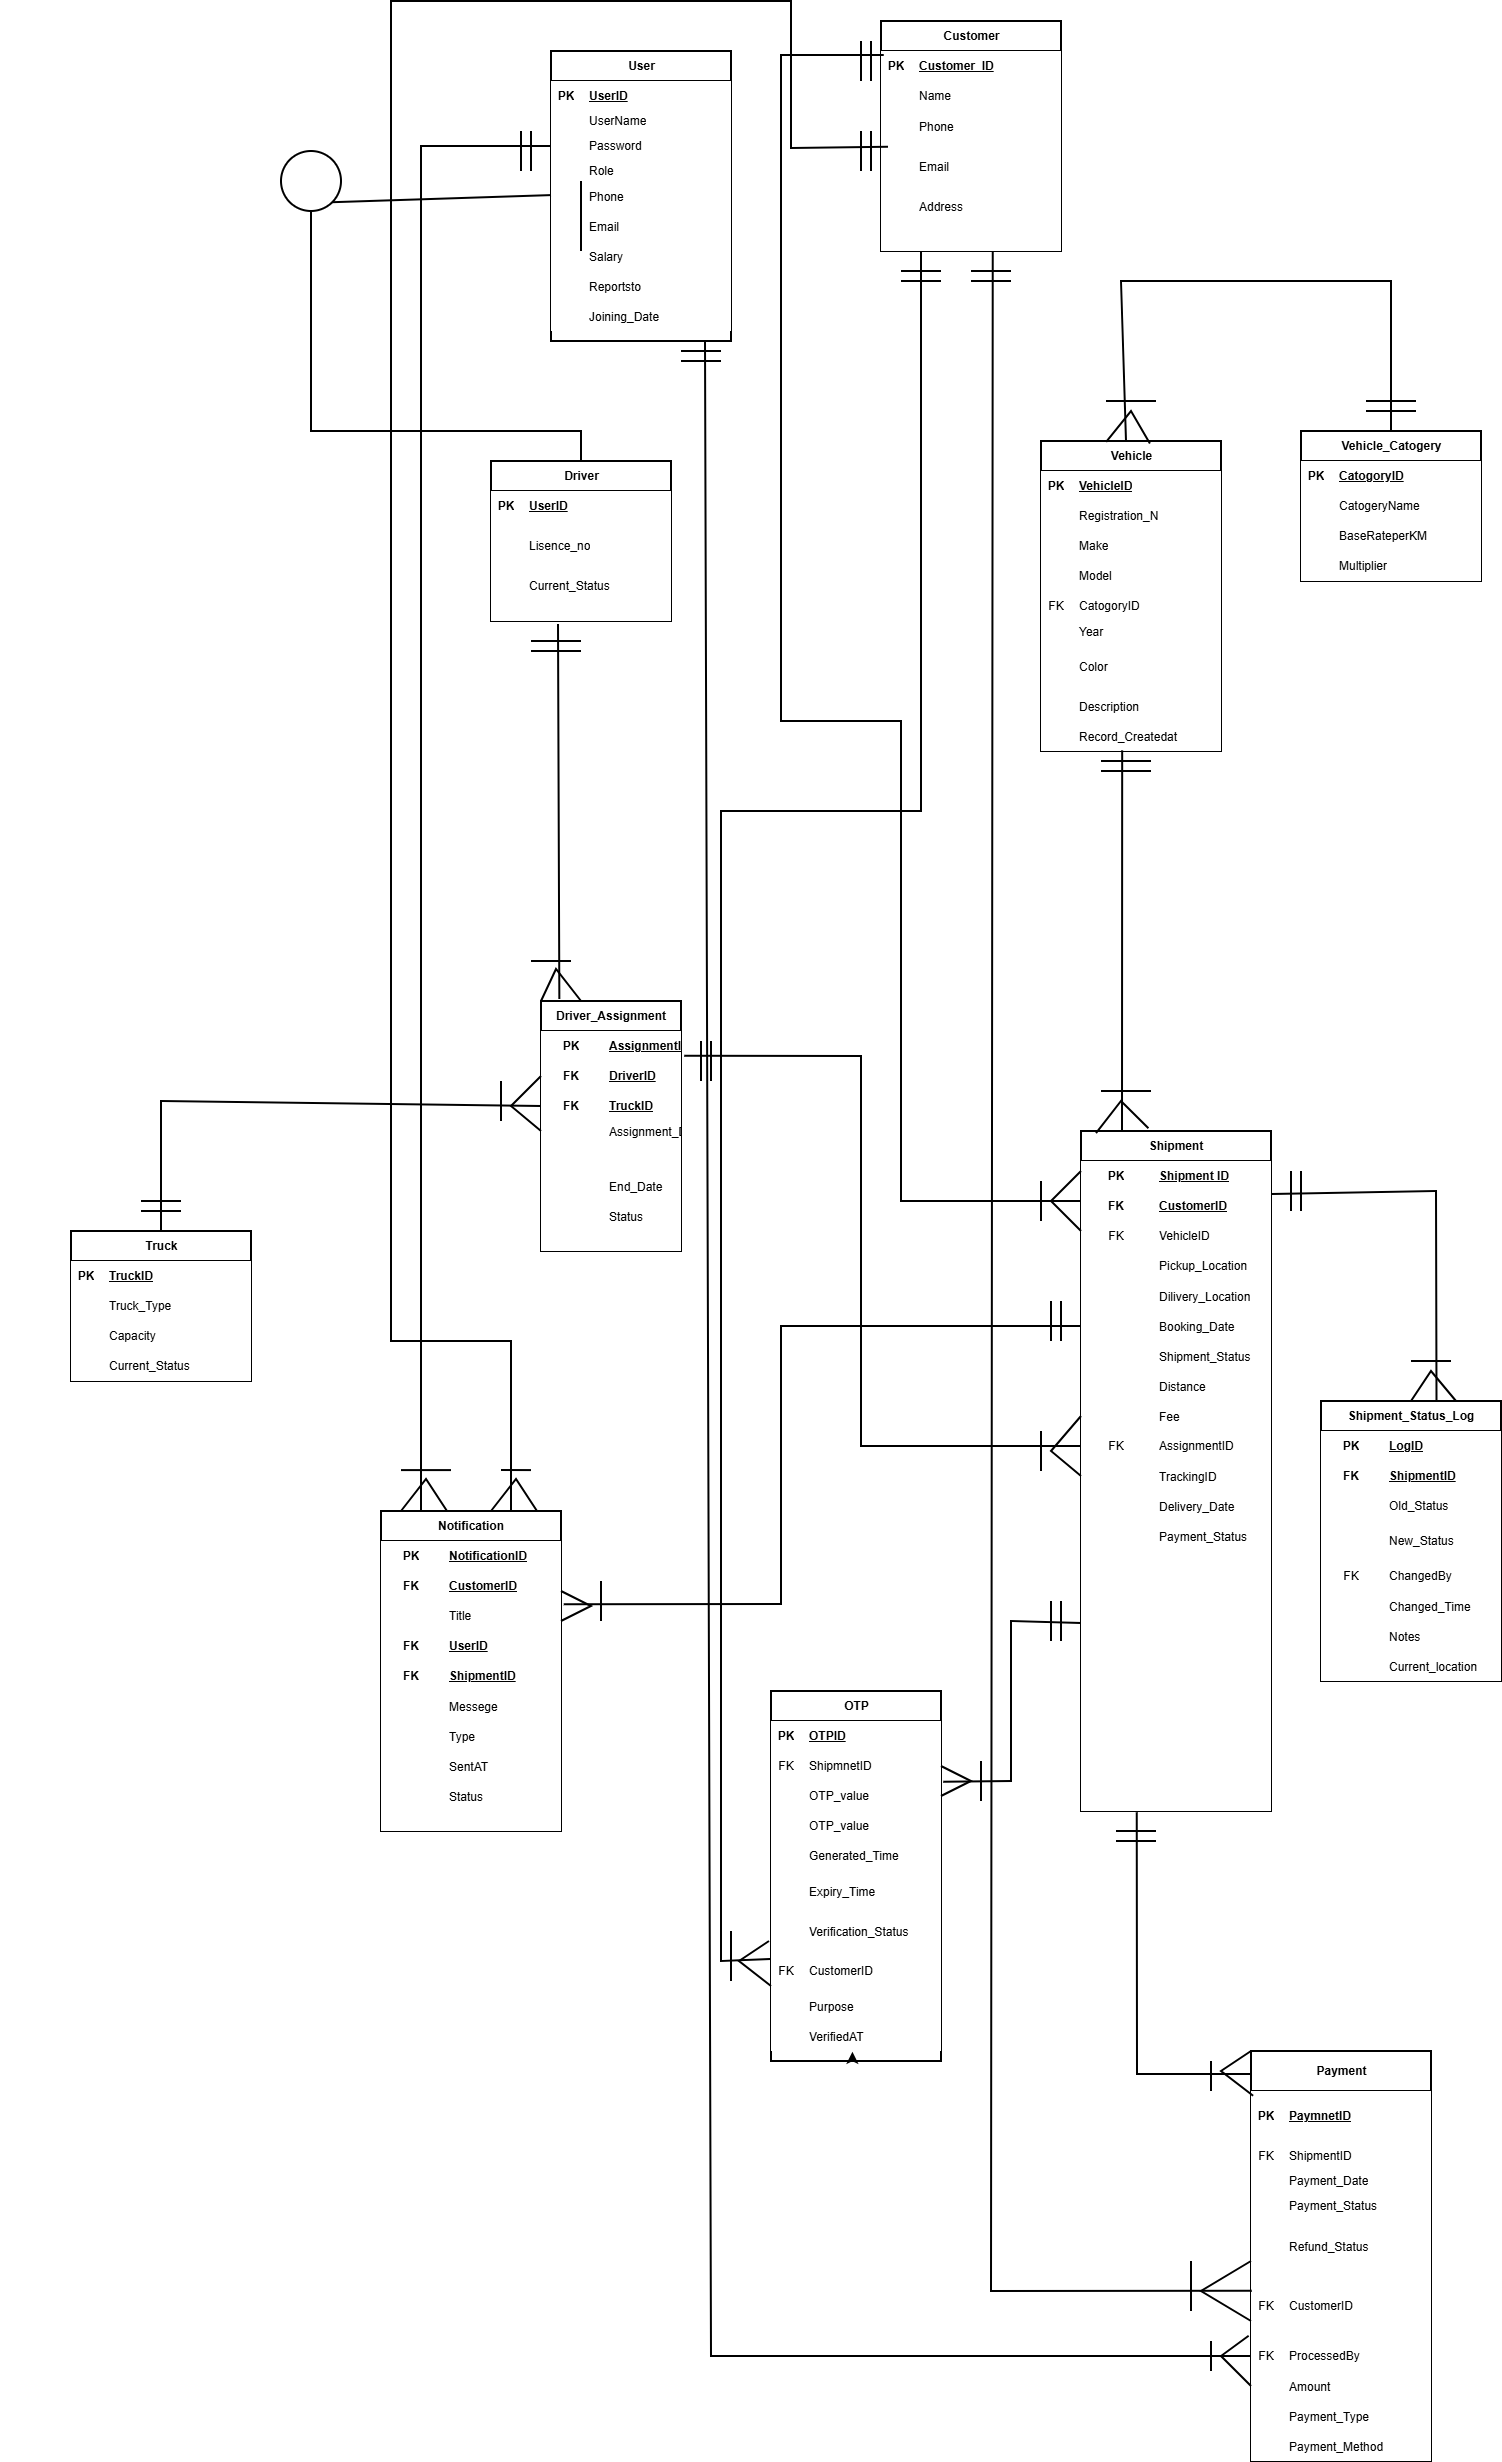
\includegraphics[width=1\linewidth]{ProjectERD.drawio.png}
    \caption{VTMS Entity Relationship Diagram (draw.io)}
\end{figure}


%------------------------------------------------
% REFERENCES
%------------------------------------------------
\chapter*{REFERENCES}

\begin{enumerate}
\item CarCarrier.pk, "Vehicle Transport Services in Pakistan," [Online]. Available: \url{https://www.carcarrier.pk}. [Accessed: April 2026].
\item Google LLC, "Google Maps Platform — Distance Matrix and Directions API Documentation," [Online]. Available: \url{https://developers.google.com/maps}. [Accessed: April 2026].
\item Jazz Telecom Pvt. Ltd., "JazzSMS API Documentation for OTP and SMS Notifications," [Online]. Available: \url{https://www.jazz.com.pk/developer}. [Accessed: April 2026].
\item JazzCash / Easypaisa, "Developer Payment Gateway and Integration APIs," [Online]. Available: \url{https://www.jazzcash.com.pk/developer}. [Accessed: April 2026].
\item Oracle Corporation, "MySQL 8.0 Reference Manual," [Online]. Available: \url{https://dev.mysql.com/doc/refman/8.0/en}. [Accessed: April 2026].
\item OpenJS Foundation, "Node.js v20 Documentation," [Online]. Available: \url{https://nodejs.org/en/docs}. [Accessed: April 2026].
\item Meta Platforms Inc., "React 18 Documentation," [Online]. Available: \url{https://react.dev}. [Accessed: April 2026].
\item diagrams.net, "draw.io ERD Diagramming Tool," [Online]. Available: \url{https://app.diagrams.net}. [Accessed: April 2026].
\item VTMS GitHub Repository, [Online]. Available: \url{https://github.com/MominaUmar74/VTMS.git}. [Accessed: April 2026].
\item OpenAI, "ChatGPT AI Assistant," Conversation Reference: \url{https://chatgpt.com/c/69b25b22-37fc-83ab-bb9f-89a521259246}. [Accessed: March–April 2026].
\end{enumerate}

%------------------------------------------------
% APPENDIX
%------------------------------------------------
\chapter*{APPENDIX: AI USAGE AND PROMPTS}

This section documents all use of AI tools during the development of the VTMS project. The table below lists each prompt submitted to an AI assistant, along with the specific purpose for which it was used.

AI Tool Used: ChatGPT (OpenAI)

Reference Conversation: \url{https://chatgpt.com/c/69b25b22-37fc-83ab-bb9f-89a521259246}

\begin{longtable}{|c|p{7cm}|p{6cm}|}
\hline
\textbf{Sr.} & \textbf{Prompt Used} & \textbf{Purpose} \\
\hline

1 & I am working on a database project for a Vehicle Transport Management System (VTMS). We have noticed that in Pakistan the manual record-keeping transport sector leads to tracking issues and payment transparency. Can you help me outline a proposal structure that covers everything from Problem Statement to Technology Stack? & Structuring the overall project proposal. Used to generate an initial framework covering all required sections. \\
\hline

2 & For our VTMS, we decided on five vehicle categories: Motorcycle, Sedan, SUV/MPV, Pickup, and Luxury. Does this cover the standard needs for a domestic export service, and what specific data attributes should we store in a MySQL table to track these shipments effectively? & Validating vehicle categories and identifying appropriate MySQL table attributes for the Vehicle and Vehicle\_Category entities. \\
\hline

3 & Our project uses Node.js and MySQL. We want to automate fee calculation using the Google Maps API and send delivery verifications via JazzSMS. How do these two APIs typically interact with a backend to update a shipment status in real time? & Understanding the API integration pattern between the Google Maps API (distance/ETA), JazzSMS API (OTP/notifications), and the Node.js/MySQL backend. \\
\hline

4 & I have drafted the conclusion for our VTMS project. Can you review it to ensure it clearly emphasises how the system increases efficiency and customer satisfaction through centralised records? & Reviewing and refining the project conclusion for clarity, completeness, and academic tone. \\
\hline

5 & We are implementing Role-Based Access Control. Can you help us define the specific database permissions for a Transport Manager versus a Finance Manager to ensure data security? & Defining and validating RBAC rules for different user roles to ensure appropriate separation of data access and system permissions. \\
\hline

\caption{AI Prompts Used and Their Purposes}
\end{longtable}

\vfill

\begin{center}
Namal University Mianwali \textbar{} Page 1 of 15
\end{center}

\end{document}